\documentclass[border=0.2cm,12pt]{standalone}
 
\usepackage{tikz}
\usetikzlibrary{positioning,automata}
\usetikzlibrary{arrows,backgrounds,calc,trees}
\usetikzlibrary{hobby} % last answer from https://tex.stackexchange.com/questions/70999/highlight-a-group-of-nodes-in-a-tikz-tree

\tikzset{>=latex} % for LaTeX arrow head
\usepackage{xcolor}

% taken from neural networks
\usepackage{amsmath} % for aligned
\usepackage{amssymb} % for \mathbb
\usepackage{listofitems} % for \readlist to create arrays
\usetikzlibrary{arrows.meta} % for arrow size
\usepackage[outline]{contour} % glow around text
\contourlength{1.4pt}

\usetikzlibrary{matrix,chains,positioning,decorations.pathreplacing,arrows}
\usetikzlibrary{shapes,arrows}
\tikzset{
  font={\fontsize{9pt}{12}\selectfont}}
\usepackage{adjustbox}
\def\layersep{3cm}

%https://tex.stackexchange.com/questions/153957/drawing-neural-network-with-tikz
\usepackage{etoolbox} % for \ifnumcomp
\tikzset{>=latex} % for LaTeX arrow head
\colorlet{myred}{red!80!black}
\colorlet{myblue}{blue!80!black}
\colorlet{mygreen}{green!60!black}
\colorlet{mydarkred}{myred!40!black}
\colorlet{mydarkblue}{myblue!40!black}
\colorlet{mydarkgreen}{mygreen!40!black}
\tikzstyle{node}=[very thick,circle,draw=myblue,minimum size=22,inner sep=0.5,outer sep=0.6]
\tikzstyle{connect}=[->,thick,mydarkblue,shorten >=1]
\tikzset{ % node styles, numbered for easy mapping with \nstyle
  node 1/.style={node,mydarkgreen,draw=mygreen,fill=mygreen!25},
  node 2/.style={node,mydarkblue,draw=myblue,fill=myblue!20},
  node 3/.style={node,mydarkred,draw=myred,fill=myred!20},
}
\def\nstyle{int(\lay<\Nnodlen?min(2,\lay):3)} % map layer number onto 1, 2, or 3


\begin{document}

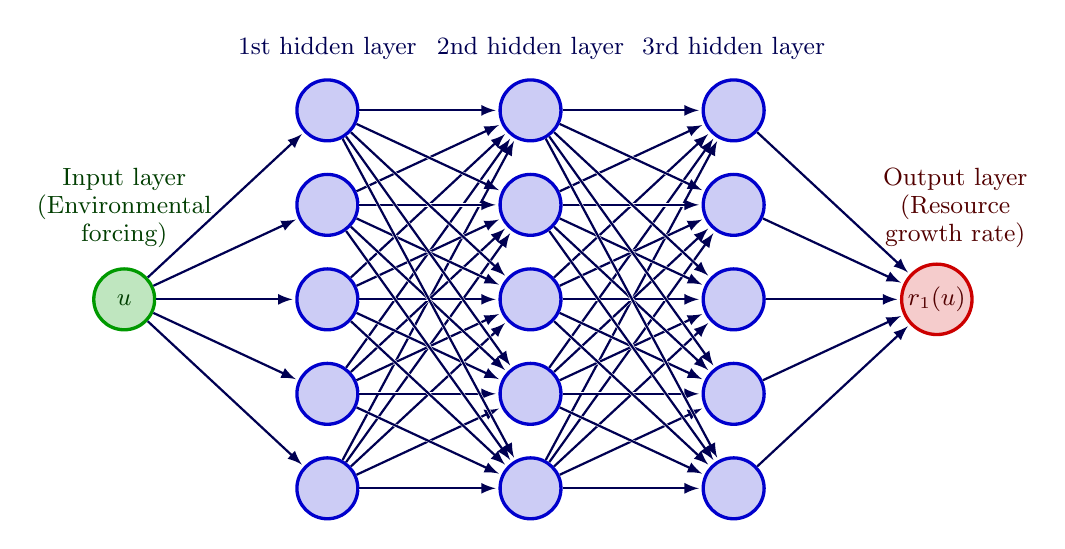
\begin{tikzpicture}[x=4.3cm,y=1.2cm]
    \readlist\Nnod{1,5,5,5,1} % array of number of nodes per layer
    \readlist\Nstr{d,d+50,} % array of string number of nodes per layer
    \readlist\Cstr{$u$,,$r_1(u)$} % array of coefficient symbol per layer
    \def\yshift{0.} % shift last node for dots
    
    % LOOP over LAYERS
    \foreachitem \N \in \Nnod{
    \def\lay{\Ncnt} % alias of index of current layer
    \pgfmathsetmacro\prev{int(\Ncnt-1)} % number of previous layer
    \foreach \i [evaluate={\c=int(\i==\N); 
                \y=\lay>0?\N/2-\i-\c*\yshift:\N/2-\i;
                \x=\lay*0.6; 
                \n=\nstyle;
                \index=(\i<\N?int(\i):"\Nstr[\n]");}] in {1,...,\N}{ % loop over nodes
        % NODES
        \node[node \n, align=center] (N\lay-\i) at (\x,\y) {\strut\Cstr[\n]};
        
        % CONNECTIONS
        \ifnumcomp{\lay}{>}{1}{ % connect to previous layer
        \foreach \j in {1,...,\Nnod[\prev]}{ % loop over nodes in previous layer
            \draw[white,line width=1.2,shorten >=1] (N\prev-\j) -- (N\lay-\i);
            \draw[connect] (N\prev-\j) -- (N\lay-\i);
        }
        }{
        % FIRST ARROWS TO GREEN NODES
        %   \draw[connect] (0.5,\y) -- (N\lay-\i); % arrows in
        }
        
    }
    % \ifnum \lay> 0
    %     \ifnum \lay<4
    %         \path (N\lay-\N) --++ (0,1+\yshift) node[midway,scale=1.6] {$\vdots$}; % dots
    %     \fi
    % \fi
    }
    
    % LABELS
    \node[above=.1,align=center,mydarkgreen] at (N1-1.90) {Input layer\\[-0.2em](Environmental\\[-0.2em]forcing)};
    \node[above=.1,align=center,mydarkblue] at (N2-1.90) {1st hidden layer};
    \node[above=.1,align=center,mydarkblue] at (N3-1.90) {2nd hidden layer};
    \node[above=.1,align=center,mydarkblue] at (N4-1.90) {3rd hidden layer};
    \node[above=.1,align=center,mydarkred] at (N\Nnodlen-1.60) {Output layer\\[-0.2em](Resource\\[-0.2em]growth rate)};
\end{tikzpicture}
\end{document}
